% Preamble templated from Mihir-Divyansh/Course-Setup
%iffalse
\let\negmedspace\undefined
\let\negthickspace\undefined
\documentclass[journal,12pt,onecolumn]{IEEEtran}
\usepackage{cite}
\usepackage{amsmath,amssymb,amsfonts,amsthm}
\usepackage{algorithmic}
\usepackage{graphicx}
\usepackage{textcomp}
\usepackage{xcolor}
\usepackage{txfonts}
\usepackage{listings}
\usepackage{enumitem}
\usepackage{mathtools}
\usepackage{gensymb}
\usepackage{comment}
\usepackage[breaklinks=true]{hyperref}
\usepackage{tkz-euclide}
\usepackage{listings}
\usepackage{gvv}
%\def\inputGnumericTable{}
\usepackage[latin1]{inputenc}
\usepackage{color}
\usepackage{array}
\usepackage{longtable}
\usepackage{calc}
\usepackage{multirow}
\usepackage{hhline}
\usepackage{ifthen}
\usepackage{lscape}
\usepackage{tabularx}
\usepackage{array}
\usepackage{float}
\usepackage{caption}
\usepackage{multicol}

\newtheorem{theorem}{Theorem}[section]
\newtheorem{problem}{Problem}
\newtheorem{proposition}{Proposition}[section]
\newtheorem{lemma}{Lemma}[section]
\newtheorem{corollary}[theorem]{Corollary}
\newtheorem{example}{Example}[section]
\newtheorem{definition}[problem]{Definition}
\newcommand{\BEQA}{\begin{eqnarray}}
\newcommand{\EEQA}{\end{eqnarray}}
\newcommand{\define}{\stackrel{\triangle}{=}}
\theoremstyle{remark}
\newtheorem{rem}{Remark}

% Marks the beginning of the document
\begin{document}
\bibliographystyle{IEEEtran}
\vspace{3cm}

\title{Assignment 2: GATE 2014 PH: Physics}
\author{EE25BTECH11055 - Subhodeep Chakraborty}
\maketitle
\hrulefill
\bigskip

\renewcommand{\thefigure}{\theenumi}
\renewcommand{\thetable}{\theenumi}

\begin{enumerate}
\item A student is required to demonstrate a high level of \underline{\smash{comprehension}} of the subject, especially in the social sciences. The word closest in meaning to \underline{\smash{comprehension}} is
% \smash to remove padding from text, making underline look closer and neater
\hfill\brak{\text{GATE PH 2014}} \begin{enumerate} \begin{multicols}{4}
    \item understanding
    \item meaning
    \item concentration
    \item stability
\end{multicols} \end{enumerate}

\item Choose the most appropriate word from the options given below to complete the following sentence. \\
One of his biggest \rule{1.5cm}{0.025pt} was his ability to forgive.
\hfill\brak{\text{GATE PH 2014}} \begin{enumerate} \begin{multicols}{4}
    \item vice
    \item virtues
    \item choices
    \item strength
\end{multicols} \end{enumerate}

\item Rajan was not happy that Sajan decided to do the project on his own. On observing his unhappiness, Sajan explained to Rajan that he preferred to work independently. Which one of the statements below is logically valid and can be inferred from the above sentences?
\hfill\brak{\text{GATE PH 2014}} \begin{enumerate}
    \item Rajan has decided to work only in a group.
    \item Rajan and Sajan were formed into a group against their wishes.
    \item Sajan had decided to give in to Rajan's request to work with him.
    \item Rajan had believed that Sajan and he would be working together.
\end{enumerate}

\item If $y = 5x^2 + 3$, then the tangent at $x = 0, y = 3$
\hfill\brak{\text{GATE PH 2014}} \begin{enumerate} \begin{multicols}{2}
    \item passes through $x = 0, y = 0$
    \item has a slope of +1
    \item is parallel to the x-axis
    \item has a slope of -1
\end{multicols} \end{enumerate}

\item A foundry has a fixed daily cost of Rs 50,000 whenever it operates and a variable cost of Rs 800Q, where Q is the daily production in tonnes. What is the cost of production in Rs per tonne for a daily production of 100 tonnes?

\item Find the odd one in the following group: ALRVX, EPVZB, ITZDF, OYEIK
\hfill\brak{\text{GATE PH 2014}} \begin{enumerate} \begin{multicols}{4}
    \item ALRVX
    \item EPVZB
    \item ITZDF
    \item OYEIK
\end{multicols} \end{enumerate}

\item Anuj, Bhola, Chandan, Dilip, Eswar and Faisal live on different floors in a six-storeyed building (the ground floor is numbered 1, the floor above it 2, and so on). Anuj lives on an even-numbered floor. Bhola does not live on an odd numbered floor. Chandan does not live on any of the floors below Faisal's floor. Dilip does not live on floor number 2. Eswar does not live on a floor immediately above or immediately below Bhola. Faisal lives three floors above Dilip. Which of the following floor-person combinations is correct?
\begin{center}
    \begin{tabular}{|c|c|c|c|c|c|c|}
    \hline
        & Anuj & Bhola & Chandan & Dilip & Eswar & Faisal \\
        \hline
        (A) & 6 & 2 & 5 & 1 & 3 & 4 \\
        \hline
        (B) & 2 & 6 & 5 & 1 & 3 & 4 \\
        \hline
        (C) & 4 & 2 & 6 & 3 & 1 & 5 \\
        \hline
        (D) & 2 & 4 & 6 & 1 & 3 & 5 \\
        \hline
    \end{tabular}
\end{center}

\item The smallest angle of a triangle is equal to two thirds of the smallest angle of a quadrilateral. The ratio between the angles of the quadrilateral is 3:4:5:6. The largest angle of the triangle is twice its smallest angle. What is the sum, in degrees, of the second largest angle of the triangle and the largest angle of the quadrilateral?

\item One percent of the people of country X are taller than 6 ft. Two percent of the people of country Y are taller than 6 ft. There are thrice as many people in country X as in country Y. Taking both countries together, what is the percentage of people taller than 6 ft?
\hfill\brak{\text{GATE PH 2014}} \begin{enumerate} \begin{multicols}{4}
    \item 3.0
    \item 2.5
    \item 1.5
    \item 1.25
\end{multicols} \end{enumerate}

\item The monthly rainfall chart based on 50 years of rainfall in Agra is shown in \figref{fig:10}.
Which of the following are true? (\textit{k} percentile is the value such that \textit{k} percent of the data fall below that value)
\begin{figure}[H]
\centering
 \caption{} \label{fig:10} 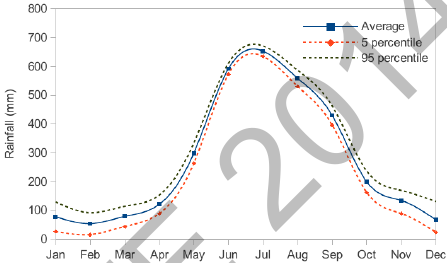
\includegraphics[width=0.8\columnwidth]{figs/q10.png}
\end{figure}

\begin{enumerate}
    \item On average, it rains more in July than in December.
    \item Every year, the amount of rainfall in August is more than that in January.
    \item July rainfall can be estimated with better confidence than February rainfall.
    \item In August, there is at least 500 mm of rainfall.
\end{enumerate}
\hfill\brak{\text{GATE PH 2014}} \begin{enumerate} \begin{multicols}{4}
    \item a and b
    \item a and c
    \item b and d
    \item c and d
\end{multicols} \end{enumerate}

\vspace{0.3cm}
\begin{center}\textbf{END OF THE QUESTION PAPER}\end{center}
\newpage

\item The unit vector perpendicular to the surface $x^2+y^2+z^2 = 3$ at the point \brak{1,1,1} is
\hfill\brak{\text{GATE PH 2014}} \begin{enumerate} \begin{multicols}{4}
    \item $\frac{\hat{x}+\hat{y}-\hat{z}}{\sqrt{3}}$
    \item $\frac{\hat{x}-\hat{y}-\hat{z}}{\sqrt{3}}$
    \item $\frac{\hat{x}-\hat{y}+\hat{z}}{\sqrt{3}}$
    \item $\frac{\hat{x}+\hat{y}+\hat{z}}{\sqrt{3}}$
\end{multicols} \end{enumerate}

\item Which one of the following quantities is invariant under Lorentz transformation?
\hfill\brak{\text{GATE PH 2014}} \begin{enumerate} \begin{multicols}{4}
    \item Charge density
    \item Charge
    \item Current
    \item Electric field
\end{multicols} \end{enumerate}

\item The number of normal Zeeman splitting components of ${}^1P \rightarrow {}^1D$ transition is
\hfill\brak{\text{GATE PH 2014}} \begin{enumerate} \begin{multicols}{4}
    \item 3
    \item 4
    \item 8
    \item 9
\end{multicols} \end{enumerate}

\item If the half-life of an elementary particle moving with speed 0.9c in the laboratory frame is $5 \times 10^{-8}$ s, then the proper half-life is \rule{3cm}{0.4pt} $\times 10^{-8}$ s. \brak{c=3\times10^8 m/s}\hfill\brak{\text{GATE PH 2014}}

\item An unpolarized light wave is incident from air on a glass surface at the Brewster angle. The angle between the reflected and the refracted wave is
\hfill\brak{\text{GATE PH 2014}} \begin{enumerate} \begin{multicols}{4}
    \item $0\degree$
    \item $45\degree$
    \item $90\degree$
    \item $120\degree$
\end{multicols} \end{enumerate}

\item Two masses m and 3m are attached to the two ends of a massless spring with force constant K. If m = 100 g and K = 0.3 N/m, then the natural angular frequency of oscillation is \rule{3cm}{0.4pt} Hz.\hfill\brak{\text{GATE PH 2014}}

\item The electric field of a uniform plane wave propagating in a dielectric, non-conducting medium is given by, $$\vec{E} = \hat{x} 10 \cos\brak{6\pi \times 10^7 t - 0.4\pi z} \, \text{V/m}$$. The phase velocity of the wave is \rule{3cm}{0.4pt} $\times 10^8$ m/s.\hfill\brak{\text{GATE PH 2014}}

\item The matrix $$A = \frac{1}{\sqrt{3}} \myvec{ 1 & 1+i \\ 1-i & -1 }$$ is
\hfill\brak{\text{GATE PH 2014}} \begin{enumerate} \begin{multicols}{4}
    \item orthogonal
    \item symmetric
    \item anti-symmetric
    \item unitary
\end{multicols} \end{enumerate}

\item The recoil momentum of an atom is $p_A$ when it emits an infrared photon of wavelength 1500 nm, and it is $p_B$ when it emits a photon of visible wavelength 500 nm. The ratio $\frac{p_A}{p_B}$ is
\hfill\brak{\text{GATE PH 2014}} \begin{enumerate} \begin{multicols}{4}
    \item 1:1
    \item $1:\sqrt{3}$
    \item 1:3
    \item 3:2
\end{multicols} \end{enumerate}

\item For a gas under isothermal conditions, its pressure P varies with volume V as $P \propto V^{-5/3}$. The bulk modulus B is proportional to
\hfill\brak{\text{GATE PH 2014}} \begin{enumerate} \begin{multicols}{4}
    \item $V^{-1/2}$
    \item $V^{-2/3}$
    \item $V^{-3/5}$
    \item $V^{-5/3}$
\end{multicols} \end{enumerate}

\item Which one of the following high energy processes is allowed by conservation laws?
\hfill\brak{\text{GATE PH 2014}} \begin{enumerate} \begin{multicols}{4}
    \item $p + \bar{p} \rightarrow \Lambda^0 + \Lambda^0$
    \item $\pi^- + p \rightarrow \pi^0 + n$
    \item $n \rightarrow p + e^- + \nu_e$
    \item $\mu^+ \rightarrow e^+ + \gamma$
\end{multicols} \end{enumerate}

\item The length element ds of an arc is given by, $\brak{ds}^2 = 2\brak{dx^1}^2 + \brak{dx^2}^2 + \sqrt{3}dx^1dx^2$. The metric tensor $g_{ij}$ is
\hfill\brak{\text{GATE PH 2014}} \begin{enumerate} \begin{multicols}{4}
    \item $\myvec{ 2 & \sqrt{3} \\ \sqrt{3} & 1 }$
    \item $\myvec{2 & \sqrt{\frac{3}{2}} \\ \sqrt{\frac{3}{2}} & 1}$
    \item $\myvec{2 & 1 \\ \sqrt{\frac{3}{2}} & \sqrt{\frac{3}{2}}}$
    \item $\myvec{1 & \sqrt{\frac{3}{2}} \\ \sqrt{\frac{3}{2}} & 2}$
\end{multicols} \end{enumerate}

\item The ground state and the first excited state wave functions of a one dimensional infinite potential well are $\psi_1$ and $\psi_2$, respectively. When two spin-up electrons are placed in this potential, which one of the following, with $x_1$ and $x_2$ denoting the position of the two electrons, correctly represents the space part of the ground state wave function of the system?
\hfill\brak{\text{GATE PH 2014}} \begin{enumerate} \begin{multicols}{2}
    \item $\frac{1}{\sqrt{2}}[\psi_1\brak{x_1}\psi_2\brak{x_1} - \psi_1\brak{x_2}\psi_2\brak{x_2}]$
    \item $\frac{1}{\sqrt{2}}[\psi_1\brak{x_1}\psi_2\brak{x_2} + \psi_1\brak{x_2}\psi_2\brak{x_1}]$
    \item $\frac{1}{\sqrt{2}}[\psi_1\brak{x_1}\psi_2\brak{x_1} + \psi_1\brak{x_2}\psi_2\brak{x_2}]$
    \item $\frac{1}{\sqrt{2}}[\psi_1\brak{x_1}\psi_2\brak{x_2} - \psi_1\brak{x_2}\psi_2\brak{x_1}]$
\end{multicols} \end{enumerate}

\item If the vector potential $$\vec{A} = \alpha x \hat{x} + 2y \hat{y} - 3z \hat{z}$$ satisfies the Coulomb gauge, the value of the constant $\alpha$ is \rule{3cm}{0.4pt}.\hfill\brak{\text{GATE PH 2014}}

\item At a given temperature, T, the average energy per particle of a non-interacting gas of two-dimensional classical harmonic oscillators is \rule{3cm}{0.4pt} $k_B T$ ($k_B$ is the Boltzmann constant).\hfill\brak{\text{GATE PH 2014}}

\item Which one of the following is a fermion?
\hfill\brak{\text{GATE PH 2014}} \begin{enumerate} \begin{multicols}{4}
    \item $\alpha$ particle
    \item ${}^7_4\text{Be}$ nucleus
    \item Hydrogen atom
    \item Deuteron
\end{multicols} \end{enumerate}

\item Which one of the following three-quark states \brak{\text{qqq}}, denoted by X, CANNOT be a possible baryon? The corresponding electric charge is indicated in the superscript.
\hfill\brak{\text{GATE PH 2014}} \begin{enumerate} \begin{multicols}{4}
    \item $X^{++}$
    \item $X^+$
    \item $X^-$
    \item $X^{--}$
\end{multicols} \end{enumerate}

\item The Hamilton's canonical equations of motion in terms of Poisson Brackets are
\hfill\brak{\text{GATE PH 2014}} \begin{enumerate} \begin{multicols}{2}
    \item $\dot{q} = \{q, H\}; \dot{p} = \{p, H\}$
    \item $\dot{q} = \{H, q\}; \dot{p} = \{H, p\}$
    \item $\dot{q} = \{H, p\}; \dot{p} = \{H, q\}$
    \item $\dot{q} = \{p, H\}; \dot{p} = \{q, H\}$
\end{multicols} \end{enumerate}

\item The Miller indices of a plane passing through the three points having coordinates \brak{0,0,1}, \brak{1,0,0}, $\brak{\frac{1}{2}, \frac{1}{2}, \frac{1}{4}}$ are
\hfill\brak{\text{GATE PH 2014}} \begin{enumerate} \begin{multicols}{4}
    \item \brak{212}
    \item \brak{111}
    \item \brak{121}
    \item \brak{211}
\end{multicols} \end{enumerate}

\item The plot of specific heat versus temperature across the superconducting transition temperature \brak{T_C} is most appropriately represented by \\
\hfill\brak{\text{GATE PH 2014}}
\begin{figure}[H]
\centering
 \caption*{} \label{fig:30o} 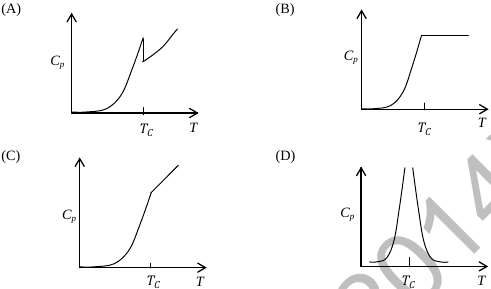
\includegraphics[width=0.8\columnwidth]{figs/q30.png}
\end{figure}

\item If $\vec{L}$ is the orbital angular momentum and $\vec{S}$ is the spin angular momentum, then $\vec{L} \cdot \vec{S}$ does NOT commute with
\hfill\brak{\text{GATE PH 2014}} \begin{enumerate} \begin{multicols}{4}
    \item $S_z$
    \item $L^2$
    \item $S^2$
    \item $\brak{\vec{L}+\vec{S}}^2$
\end{multicols} \end{enumerate}

\item The energy, $\epsilon_k$ for band electrons as a function of the wave vector, k in the first Brillouin zone \brak{-\pi/a \le k \le \pi/a} of a one dimensional monatomic lattice is shown in \figref{fig:32} (a is lattice constant).
\begin{figure}[H]
\centering
 \caption{} \label{fig:32} 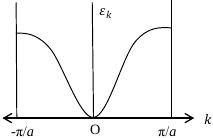
\includegraphics[width=0.3\columnwidth]{figs/q32.png}
\end{figure}
The variation of the group velocity $v_k$ is most appropriately represented by
\hfill\brak{\text{GATE PH 2014}}
\begin{figure}[H]
\centering
 \caption*{} \label{fig:32o} 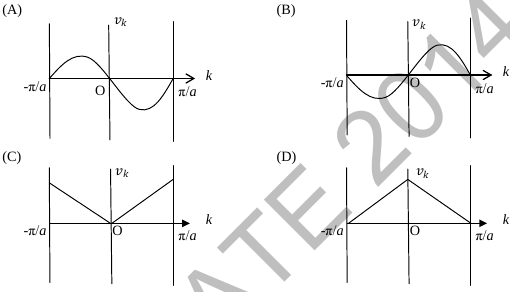
\includegraphics[width=0.8\columnwidth]{figs/q32o.png}
\end{figure}
\item For a free electron gas in two dimensions, the variation of the density of states, N(E) as a function of energy E, is best represented by
\hfill\brak{\text{GATE PH 2014}}
\begin{figure}[H]
\centering
 \caption*{} \label{fig:33o} 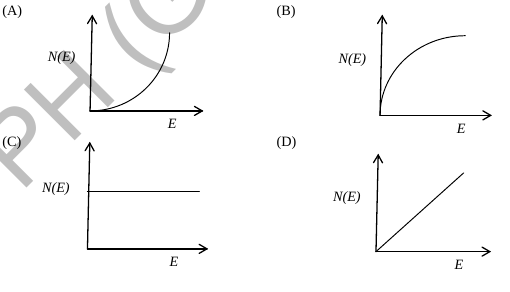
\includegraphics[width=0.8\columnwidth]{figs/q33.png}
\end{figure}
\item The input given to an ideal OP-AMP integrator circuit is shown in \figref{fig:34}
\begin{figure}[H]
\centering
 \caption{} \label{fig:34} 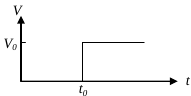
\includegraphics[width=0.25\columnwidth]{figs/q34.png}
\end{figure}
The correct output of the integrator circuit is
\hfill\brak{\text{GATE PH 2014}}
\begin{figure}[H]
\centering
 \caption*{} \label{fig:34o} 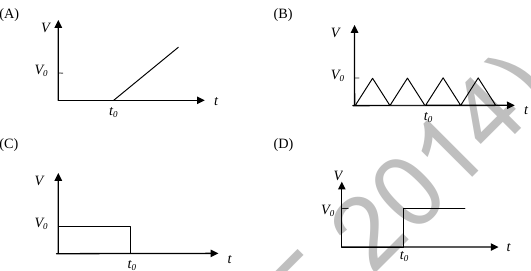
\includegraphics[width=0.7\columnwidth]{figs/q34o.png}
\end{figure}
\item The minimum number of flip-flops required to construct a mod-75 counter is \rule{3cm}{0.4pt}.\hfill\brak{\text{GATE PH 2014}}

\item A bead of mass m can slide without friction along a massless rod kept at 45$\degree$ with the vertical as shown in \figref{fig:36}. The rod is rotating about the vertical axis with a constant angular speed $\omega$. At any instant, r is the distance of the bead from the origin. The momentum conjugate to r is
\begin{figure}[H]
\centering
 \caption{} \label{fig:36} 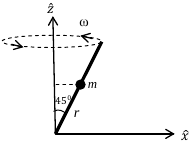
\includegraphics[width=0.3\columnwidth]{figs/q36.png}
\end{figure}
\hfill\brak{\text{GATE PH 2014}} \begin{enumerate} \begin{multicols}{4}
    \item $m\dot{r}$
    \item $\frac{1}{2}m\dot{r}$
    \item $\frac{1}{2}m\dot{r}$
    \item $2m\dot{r}$
\end{multicols} \end{enumerate}

\item An electron in the ground state of the hydrogen atom has the wave function $$\Psi\brak{\vec{r}} = \frac{1}{\sqrt{\pi a_0^3}} e^{-\brak{r/a_0}}$$ where $a_0$ is constant. The expectation value of the operator $\hat{Q} = z^2 - r^2$, where $z = r\cos\theta$ is (Hint: $\int_0^\infty e^{-\alpha r} r^n dr = \frac{\Gamma(n)}{\alpha^{n+1}} = \frac{(n-1)!}{\alpha^{n+1}}$)
\hfill\brak{\text{GATE PH 2014}} \begin{enumerate} \begin{multicols}{4}
    \item $-a_0^2/2$
    \item $-a_0^2$
    \item $-3a_0^2/2$
    \item $-2a_0^2$
\end{multicols} \end{enumerate}

\item For Nickel, the number density is $8 \times 10^{23} \text{ atoms}/cm^3$ and electronic configuration is $1s^22s^22p^63s^23p^63d^84s^2$. The value of the saturation magnetization of Nickel in its ferromagnetic state is \rule{3cm}{0.4pt} $\times 10^9 A/m$. (Given the value of Bohr magneton $\mu_B = 9.21 \times 10^{-21} Am^2$)\hfill\brak{\text{GATE PH 2014}}

\item A particle of mass m is in a potential given by $$V(r) = -\frac{a}{r} + \frac{ar_0^2}{3r^3}$$, where a and $r_0$ are positive constants. When disturbed slightly from its stable equilibrium position, it undergoes a simple harmonic oscillation. The time period of oscillation is
\hfill\brak{\text{GATE PH 2014}} \begin{enumerate} \begin{multicols}{4}
    \item $2\pi \sqrt{\frac{mr_0^3}{2a}}$
    \item $2\pi \sqrt{\frac{mr_0^3}{a}}$
    \item $2\pi \sqrt{\frac{2mr_0^3}{a}}$
    \item $4\pi \sqrt{\frac{mr_0^3}{a}}$
\end{multicols} \end{enumerate}

\item The donor concentration in a sample of n-type silicon is increased by a factor of 100. The shift in the position of the Fermi level at 300K, assuming the sample to be non degenerate is \rule{3cm}{0.4pt} meV. \brak{k_B T = 25 \text{ meV} \text{at 300 K}}\hfill\brak{\text{GATE PH 2014}}

\item A particle of mass $m$ is subjected to a potential, $$V(x,y) = \frac{1}{2} m\omega^2(x^2+y^2), -\infty \le x \le \infty, -\infty \le y \le \infty$$. The state with energy $4\hbar\omega$ is $g$-fold degenerate. The value of $g$ is \rule{3cm}{0.4pt}.\hfill\brak{\text{GATE PH 2014}}

\item A hydrogen atom is in the state $$\Psi = \sqrt{\frac{8}{21}}\psi_{200} - \sqrt{\frac{3}{7}}\psi_{310} + \sqrt{\frac{4}{21}}\psi_{321}$$, where $n,l,m$ in $\psi_{nlm}$ denote the principal, orbital and magnetic quantum numbers, respectively. If $\vec{L}$ is the angular momentum operator, the average value of $L^2$ is \rule{3cm}{0.4pt} $\hbar^2$.\hfill\brak{\text{GATE PH 2014}}

\item A planet of mass m moves in a circular orbit of radius $r_0$ in the gravitational potential $V(r) = -k/r$, where k is a positive constant. The orbital angular momentum of the planet is
\hfill\brak{\text{GATE PH 2014}} \begin{enumerate} \begin{multicols}{4}
    \item $2r_0km$
    \item $\sqrt{2r_0km}$
    \item $r_0km$
    \item $\sqrt{r_0km}$
\end{multicols} \end{enumerate}

\item The moment of inertia of a rigid diatomic molecule A is 6 times that of another rigid diatomic molecule B. If the rotational energies of the two molecules are equal, then the corresponding values of the rotational quantum numbers $J_A$ and $J_B$ are
\hfill\brak{\text{GATE PH 2014}} \begin{enumerate} \begin{multicols}{4}
    \item $J_A = 2, J_B = 1$
    \item $J_A = 3, J_B = 1$
    \item $J_A = 5, J_B = 0$
    \item $J_A = 6, J_B = 1$
\end{multicols} \end{enumerate}

\item The value of the integral $$\oint\limits_C \frac{z^2}{e^z+1} dz$$, where C is the circle $|z|=4$, is
\hfill\brak{\text{GATE PH 2014}} \begin{enumerate} \begin{multicols}{4}
    \item $2\pi i$
    \item $2\sqrt{2}\pi i$
    \item $4\pi i / 3$
    \item $4\pi i / \sqrt{2}$
\end{multicols} \end{enumerate}

\item A ray of light inside Region 1 in the xy-plane is incident at the semicircular boundary that carries no free charges. The electric field at the point $P(r_0, \pi/4)$ in plane polar coordinates is $\vec{E}_1 = 7\hat{e}_r - 3\hat{e}_\phi$, where $\hat{e}_r$ and $\hat{e}_\phi$ are the unit vectors. The emerging ray in Region 2 has the electric field $\vec{E}_2$ parallel to x-axis. If $\epsilon_1$ and $\epsilon_2$ are the dielectric constants of Region 1 and Region 2 respectively, then $\frac{\epsilon_2}{\epsilon_1}$ is \rule{5cm}{0.4pt}
\hfill\brak{\text{GATE PH 2014}}
\begin{figure}[H]
\centering
 \caption*{} \label{fig:46} 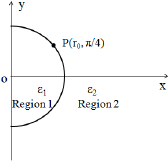
\includegraphics{figs/q46.png}
\end{figure}
\item The solution of the differential equation $$\frac{d^2y}{dt^2} - y = 0$$, subject to the boundary conditions $y(0)=1$ and $y(\infty)=0$, is
\hfill\brak{\text{GATE PH 2014}} \begin{enumerate} \begin{multicols}{4}
    \item $\cos t + \sin t$
    \item $\cosh t + \sinh t$
    \item $\cos t - \sin t$
    \item $\cosh t - \sinh t$
\end{multicols} \end{enumerate}

\item Given that the linear transformation of a generalized coordinate q and the corresponding momentum p, $$Q = q + 4ap, \\P = q + 2p$$ is canonical, the value of the constant a is \rule{3cm}{0.4pt}.\hfill\brak{\text{GATE PH 2014}}

\item The value of the magnetic field required to maintain non-relativistic protons of energy 1 MeV in a circular orbit of radius 100 mm is \rule{4cm}{0.4pt} Tesla. \brak{\text{Given: $m_p = 1.67 \times 10^{-27} \text{kg}$, $e = 1.6 \times 10^{-19} \text{C}$}}\hfill\brak{\text{GATE PH 2014}}

\item For a system of two bosons, each of which can occupy any of the two energy levels 0 and $\epsilon$, the mean energy of the system at a temperature T with $\beta = \frac{1}{k_BT}$ is given by
\hfill\brak{\text{GATE PH 2014}} \begin{enumerate} \begin{multicols}{2}
    \item $\frac{\epsilon e^{-\beta\epsilon} + 2\epsilon e^{-2\beta\epsilon}}{1+2e^{-\beta\epsilon}+e^{-2\beta\epsilon}} $
    \item $\frac{1+\epsilon e^{-\beta\epsilon}}{2e^{-\beta\epsilon}+e^{-2\beta\epsilon}}$
    \item $\frac{2\epsilon e^{-\beta\epsilon}+\epsilon e^{-2\beta\epsilon}}{2+e^{-\beta\epsilon}+e^{-2\beta\epsilon}}$
    \item $\frac{\epsilon e^{-\beta\epsilon}+2\epsilon e^{-2\beta\epsilon}}{2+e^{-\beta\epsilon}+e^{-2\beta\epsilon}}$
\end{multicols} \end{enumerate}

\item In an interference pattern formed by two coherent sources, the maximum and the minimum of the intensities are $9I_0$ and $I_0$, respectively. The intensities of the individual waves are
\hfill\brak{\text{GATE PH 2014}} \begin{enumerate} \begin{multicols}{4}
    \item $3I_0$ and $I_0$
    \item $4I_0$ and $I_0$
    \item $5I_0$ and $4I_0$
    \item $9I_0$ and $I_0$
\end{multicols} \end{enumerate}

\item $\psi_1$ and $\psi_2$ are two orthogonal states of a spin $1/2$ system. It is given that $$\psi_1 = \frac{1}{\sqrt{3}} \myvec{ 1 \\ 0 } + \frac{\sqrt{2}}{\sqrt{3}} \myvec{ 0 \\ 1 }$$, where $\myvec{1 \\ 0}$ and $\myvec{0 \\ 1}$ represent the spin-up and spin-down states, respectively. When the system is in the state $\psi_2$, its probability to be in the spin-up state is \rule{3cm}{0.4pt}.\hfill\brak{\text{GATE PH 2014}}

\item Neutrons moving with speed $10^3$ m/s are used for the determination of crystal structure. If the Bragg angle for the first order diffraction is $30\degree$, the interplanar spacing of the crystal is \rule{3cm}{0.4pt} \AA. (Given: $m_n = 1.675 \times 10^{-27}$ kg, $h = 6.626 \times 10^{-34}$ J.s)\hfill\brak{\text{GATE PH 2014}}

\item The Hamiltonian of a particle of mass m is given by $H = \frac{p^2}{2m} - \frac{\alpha q^2}{2}$. Which one of the following figures describes the motion of the particle in phase space?
\hfill\brak{\text{GATE PH 2014}}
\begin{figure}[H]
\centering
 \caption*{} \label{fig:54} 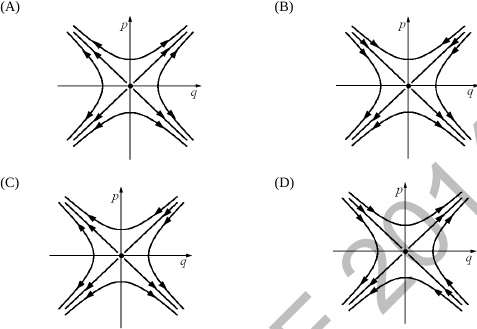
\includegraphics{figs/q54.png}
\end{figure}
\item The intensity of a laser in free space is 150 mW/m$^2$. The corresponding amplitude of the electric field of the laser is \rule{3cm}{0.4pt} V/m. \brak{\epsilon_0 = 8.854 \times 10^{-12} C^2/N.m^2}\hfill\brak{\text{GATE PH 2014}}

\item The emission wavelength for the transition ${}^1D_2 \rightarrow {}^1F_3$ is 3122 \AA. The ratio of populations of the final to the initial states at a temperature 5000 K is \brak{h = 6.626 \times 10^{-34} \text{J.s}, c = 3 \times 10^8 \text{m/s}, k_B = 1.380 \times 10^{-23} \text{J/K}}
\hfill\brak{\text{GATE PH 2014}} \begin{enumerate} \begin{multicols}{4}
    \item $2.03 \times 10^{-5}$
    \item $4.02 \times 10^{-5}$
    \item $7.02 \times 10^{-5}$
    \item $9.83 \times 10^{-5}$
\end{multicols} \end{enumerate}

\item Consider a system of 3 fermions, which can occupy any of the 4 available energy states with equal probability. The entropy of the system is
\hfill\brak{\text{GATE PH 2014}} \begin{enumerate} \begin{multicols}{4}
    \item $k_B \ln 2$
    \item $2 k_B \ln 2$
    \item $2 k_B \ln 4$
    \item $3 k_B \ln 4$
\end{multicols} \end{enumerate}

\item A particle is confined to a one dimensional potential box with the potential
\[ V(x) = \begin{cases} 0, & 0 < x < a \\ \infty, & \text{otherwise} \end{cases} \]
If the particle is subjected to a perturbation, within the box, $W = \beta x$, where $\beta$ is a small constant, the first order correction to the ground state energy is
\hfill\brak{\text{GATE PH 2014}} \begin{enumerate} \begin{multicols}{4}
    \item 0
    \item $\alpha\beta /4$
    \item $\alpha\beta /2$
    \item $\alpha\beta $
\end{multicols} \end{enumerate}

\item Consider the process $\mu^+ + \mu^- \rightarrow \pi^+ + \pi^-$. The minimum kinetic energy of the muons \brak{\mu} in the centre of mass frame required to produce the pion \brak{\pi} pairs at rest is \rule{3cm}{0.4pt} MeV. (Given: $m_\mu = 105 \text{ MeV/c}^2$, $m_\pi = 140 \text{ MeV/c}^2$).\hfill\brak{\text{GATE PH 2014}}

\item A one dimensional harmonic oscillator is in the superposition of number states, $|n\rangle$, given by $$|\psi\rangle = \frac{1}{2}|1\rangle + \frac{\sqrt{3}}{2}|2\rangle + \frac{\sqrt{3}}{2}|3\rangle$$. The average energy of the oscillator in the given state is \rule{3cm}{0.4pt} $\hbar\omega$.\hfill\brak{\text{GATE PH 2014}}

\item A nucleus X undergoes a first forbidden $\beta$-decay to a nucleus Y. If the angular momentum (I) and parity (P), denoted by $I^P$ as $7/2^-$ for X, which of the following is a possible $I^P$ value for Y?
\hfill\brak{\text{GATE PH 2014}} \begin{enumerate} \begin{multicols}{4}
    \item $1/2^+$
    \item $1/2^-$
    \item $3/2^+$
    \item $3/2^-$
\end{multicols} \end{enumerate}

\item The current gain of the transistor in the following circuit in \figref{fig:62} is $\beta_{dc} = 100$. The value of collector current $I_c$ is \rule{3cm}{0.4pt} mA.
\hfill\brak{\text{GATE PH 2014}}
\begin{figure}[H]
\centering
 \caption{} \label{fig:62} 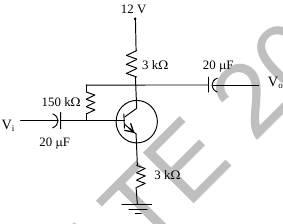
\includegraphics{figs/q62.png}
\end{figure}
\item In order to measure a maximum of 1V with a resolution of 1mV using a n-bit A/D converter, working under the principle of ladder network, the minimum value of n is \rule{3cm}{0.4pt}.\hfill\brak{\text{GATE PH 2014}}

\item If $L_+$ and $L_-$ are the angular momentum ladder operators, then, the expectation value of $\brak{L_+L_- + L_-L_+}$, in the state $|l=1, m=1\rangle$ of an atom is \rule{3cm}{0.4pt} $\hbar^2$.\hfill\brak{\text{GATE PH 2014}}

\item A low pass filter is formed by a resistance R and a capacitance C. At the cut-off angular frequency $\omega_c = 1/RC$, the voltage gain and the phase of the output voltage relative to the input voltage respectively, are
\hfill\brak{\text{GATE PH 2014}} \begin{enumerate} \begin{multicols}{4}
    \item 0.71 and $45\degree$
    \item 0.71 and $-45\degree$
    \item 0.5 and $-90\degree$
    \item 0.5 and $90\degree$
\end{multicols} \end{enumerate}
\end{enumerate}

\hrulefill
\textbf{END OF THE QUESTION PAPER}
\hrulefill

\end{document}
